\documentclass[9pt,twocolumn,twoside,]{pnas-new}

% Use the lineno option to display guide line numbers if required.
% Note that the use of elements such as single-column equations
% may affect the guide line number alignment.


\usepackage[T1]{fontenc}
\usepackage[utf8]{inputenc}
% Pandoc syntax highlighting
\usepackage{color}
\usepackage{fancyvrb}
\newcommand{\VerbBar}{|}
\newcommand{\VERB}{\Verb[commandchars=\\\{\}]}
\DefineVerbatimEnvironment{Highlighting}{Verbatim}{commandchars=\\\{\}}
% Add ',fontsize=\small' for more characters per line
\newenvironment{Shaded}{}{}
\newcommand{\AlertTok}[1]{\textcolor[rgb]{1.00,0.00,0.00}{\textbf{#1}}}
\newcommand{\AnnotationTok}[1]{\textcolor[rgb]{0.38,0.63,0.69}{\textbf{\textit{#1}}}}
\newcommand{\AttributeTok}[1]{\textcolor[rgb]{0.49,0.56,0.16}{#1}}
\newcommand{\BaseNTok}[1]{\textcolor[rgb]{0.25,0.63,0.44}{#1}}
\newcommand{\BuiltInTok}[1]{#1}
\newcommand{\CharTok}[1]{\textcolor[rgb]{0.25,0.44,0.63}{#1}}
\newcommand{\CommentTok}[1]{\textcolor[rgb]{0.38,0.63,0.69}{\textit{#1}}}
\newcommand{\CommentVarTok}[1]{\textcolor[rgb]{0.38,0.63,0.69}{\textbf{\textit{#1}}}}
\newcommand{\ConstantTok}[1]{\textcolor[rgb]{0.53,0.00,0.00}{#1}}
\newcommand{\ControlFlowTok}[1]{\textcolor[rgb]{0.00,0.44,0.13}{\textbf{#1}}}
\newcommand{\DataTypeTok}[1]{\textcolor[rgb]{0.56,0.13,0.00}{#1}}
\newcommand{\DecValTok}[1]{\textcolor[rgb]{0.25,0.63,0.44}{#1}}
\newcommand{\DocumentationTok}[1]{\textcolor[rgb]{0.73,0.13,0.13}{\textit{#1}}}
\newcommand{\ErrorTok}[1]{\textcolor[rgb]{1.00,0.00,0.00}{\textbf{#1}}}
\newcommand{\ExtensionTok}[1]{#1}
\newcommand{\FloatTok}[1]{\textcolor[rgb]{0.25,0.63,0.44}{#1}}
\newcommand{\FunctionTok}[1]{\textcolor[rgb]{0.02,0.16,0.49}{#1}}
\newcommand{\ImportTok}[1]{#1}
\newcommand{\InformationTok}[1]{\textcolor[rgb]{0.38,0.63,0.69}{\textbf{\textit{#1}}}}
\newcommand{\KeywordTok}[1]{\textcolor[rgb]{0.00,0.44,0.13}{\textbf{#1}}}
\newcommand{\NormalTok}[1]{#1}
\newcommand{\OperatorTok}[1]{\textcolor[rgb]{0.40,0.40,0.40}{#1}}
\newcommand{\OtherTok}[1]{\textcolor[rgb]{0.00,0.44,0.13}{#1}}
\newcommand{\PreprocessorTok}[1]{\textcolor[rgb]{0.74,0.48,0.00}{#1}}
\newcommand{\RegionMarkerTok}[1]{#1}
\newcommand{\SpecialCharTok}[1]{\textcolor[rgb]{0.25,0.44,0.63}{#1}}
\newcommand{\SpecialStringTok}[1]{\textcolor[rgb]{0.73,0.40,0.53}{#1}}
\newcommand{\StringTok}[1]{\textcolor[rgb]{0.25,0.44,0.63}{#1}}
\newcommand{\VariableTok}[1]{\textcolor[rgb]{0.10,0.09,0.49}{#1}}
\newcommand{\VerbatimStringTok}[1]{\textcolor[rgb]{0.25,0.44,0.63}{#1}}
\newcommand{\WarningTok}[1]{\textcolor[rgb]{0.38,0.63,0.69}{\textbf{\textit{#1}}}}

% tightlist command for lists without linebreak
\providecommand{\tightlist}{%
  \setlength{\itemsep}{0pt}\setlength{\parskip}{0pt}}

% From pandoc table feature
\usepackage{longtable,booktabs,array}
\usepackage{calc} % for calculating minipage widths
% Correct order of tables after \paragraph or \subparagraph
\usepackage{etoolbox}
\makeatletter
\patchcmd\longtable{\par}{\if@noskipsec\mbox{}\fi\par}{}{}
\makeatother
% Allow footnotes in longtable head/foot
\IfFileExists{footnotehyper.sty}{\usepackage{footnotehyper}}{\usepackage{footnote}}
\makesavenoteenv{longtable}



\templatetype{pnasmathematics}  % Choose template

\title{Problem Set 1}

\author[]{Carlos Enrique Lezama Jacinto}

  \affil[]{Instituto Tecnológico Autónomo de México}


% Please give the surname of the lead author for the running footer
\leadauthor{}

% Please add here a significance statement to explain the relevance of your work
\significancestatement{}


\authorcontributions{}



\correspondingauthor{\textsuperscript{} My solutions to the first
problem set in Advanced Microeconometrics (ECO -- 20513).}

% Keywords are not mandatory, but authors are strongly encouraged to provide them. If provided, please include two to five keywords, separated by the pipe symbol, e.g:


\begin{abstract}

\end{abstract}

\dates{This manuscript was compiled on \today}
\doi{\url{www.pnas.org/cgi/doi/10.1073/pnas.XXXXXXXXXX}}

\begin{document}

% Optional adjustment to line up main text (after abstract) of first page with line numbers, when using both lineno and twocolumn options.
% You should only change this length when you've finalised the article contents.
\verticaladjustment{-2pt}



\maketitle
\thispagestyle{firststyle}
\ifthenelse{\boolean{shortarticle}}{\ifthenelse{\boolean{singlecolumn}}{\abscontentformatted}{\abscontent}}{}

% If your first paragraph (i.e. with the \dropcap) contains a list environment (quote, quotation, theorem, definition, enumerate, itemize...), the line after the list may have some extra indentation. If this is the case, add \parshape=0 to the end of the list environment.

\acknow{}

\newcommand{\ind}{\perp\!\!\!\!\perp}

\hypertarget{the-model}{%
\section*{The Model}\label{the-model}}
\addcontentsline{toc}{section}{The Model}

Assume that the economic model generating the data for potential
outcomes is of the form:

\begin{align*}
Y_1 &= \alpha + \varphi + U_1, \\
Y_0 &= \alpha + U_0,
\end{align*}

where \(U_1\) and \(U_0\) represent the unobservables in the potential
outcome equations and \(\varphi\) represents the benefit associated with
the treatment (\(D = 1\)). Individuals decide whether or not to receive
the treatment (\(D = 1\) or \(D = 0\)) based on a latent variable \(I\):

\[
I = Z \gamma + V,
\]

where \(Z\) and \(V\) represent observables and unobservables,
respectively. Thus, we can define a binary variable \(D\) indicating
treatment status,

\[
D = \mathds{1}\left[ I \geq 0\right].
\]

Finally, we assume that the error terms in the model are not independent
even conditioning on the observables,
i.e.~\(U_1 \not\perp\!\!\!\!\perp U_0 \not\perp\!\!\!\!\perp V \mid Z\),
but \((U_1, U_0, V) \perp\!\!\!\!\perp Z\).

\hypertarget{treatment-parameters}{%
\section{Treatment Parameters}\label{treatment-parameters}}

Let \(\beta = Y_1 - Y_0 = \varphi + U_1 - U_0\) such that, in regression
notation, \(Y = \alpha + \beta D + \varepsilon\) where
\(\varepsilon = U_0\).

\hypertarget{average-treatment-effect}{%
\subsection*{Average Treatment Effect}\label{average-treatment-effect}}
\addcontentsline{toc}{subsection}{Average Treatment Effect}

\begin{align*}
ATE &= E \left[ \beta \right] \\
&= E \left[ \varphi + U_1 - U_0 \right] \\
&= \varphi
\end{align*}

\hypertarget{treatment-on-the-treated}{%
\subsection*{Treatment on the Treated}\label{treatment-on-the-treated}}
\addcontentsline{toc}{subsection}{Treatment on the Treated}

\begin{align*}
TT &= E \left[ \beta \mid D = 1 \right] \\
&= E \left[ \varphi + U_1 - U_0 \mid Z \gamma + V \geq 0 \right] \\
&= \varphi + E \left[ U_1 - U_0 \mid V \geq - Z \gamma \right]
\end{align*}

\hypertarget{treatment-on-the-untreated}{%
\subsection*{Treatment on the
Untreated}\label{treatment-on-the-untreated}}
\addcontentsline{toc}{subsection}{Treatment on the Untreated}

\begin{align*}
TUT &= E \left[ \beta \mid D = 0 \right] \\
&= E \left[ \varphi + U_1 - U_0 \mid Z \gamma + V < 0 \right] \\
&= \varphi + E \left[ U_1 - U_0 \mid V < - Z \gamma \right]
\end{align*}

\hypertarget{marginal-treatment-effect}{%
\subsection*{Marginal Treatment
Effect}\label{marginal-treatment-effect}}
\addcontentsline{toc}{subsection}{Marginal Treatment Effect}

\begin{align*}
MTE &= E \left[ \beta \mid I = 0,\ V = v \right] \\
&= E \left[ \varphi + U_1 - U_0 \mid I = 0,\ V = v \right] \\
&= \varphi + E \left[ U_1 - U_0 \mid Z \gamma = - V,\ V = v \right]
\end{align*}

\hypertarget{instrumental-variables}{%
\subsection*{Instrumental Variables}\label{instrumental-variables}}
\addcontentsline{toc}{subsection}{Instrumental Variables}

\[
\hat{\beta}_{\text{IV}} (J(Z)) = \frac{\text{Cov}(J(Z), Y)}{\text{Cov}(J(Z), D)} \overset{p}{\longrightarrow} \beta
\]

\hypertarget{ordinary-least-squares}{%
\subsection*{Ordinary Least Squares}\label{ordinary-least-squares}}
\addcontentsline{toc}{subsection}{Ordinary Least Squares}

\[
\hat{\beta}_{\text{OLS}} = \frac{\text{Cov}(Y, D)}{\text{Var}(D)} \implies \hat{\beta}_{\text{OLS}} = \left( D^T D \right)^{-1} D^T Y
\]

\hypertarget{local-average-treatment-effect}{%
\subsection*{Local Average Treatment
Effect}\label{local-average-treatment-effect}}
\addcontentsline{toc}{subsection}{Local Average Treatment Effect}

\begin{align*}
LATE &= E \left[ \beta \mid D(z) = 0, D(z') = 1 \right] \\
&= E \left[ \beta \mid z \gamma < - V \leq z' \gamma \right] \\
&= \varphi + E \left[ U_1 - U_0 \mid - z' \gamma \leq V < - z \gamma \right]
\end{align*}

\hypertarget{some-closed-form-expressions}{%
\section{Some closed form
expressions}\label{some-closed-form-expressions}}

Suppose that the error terms in the model have the following structure:

\begin{align*}
U_1 &= \sigma_1 \epsilon, \\
U_0 &= \sigma_0 \epsilon, \\
V &= \sigma^*_V \epsilon, \\
\epsilon &\sim \mathcal{N} (0, 1).
\end{align*}

So, we can say that

\begin{align*}
TT &= \varphi + E \left[ U_1 - U_0 \mid V \geq - Z \gamma \right] \\
&= \varphi + E \left[ \epsilon (\sigma_1 - \sigma_0) \mid \epsilon \geq \frac{- Z \gamma}{\sigma^*_V} \right] \\
&= \varphi + (\sigma_1 - \sigma_0) E \left[ \epsilon \mid \epsilon \geq \frac{- Z \gamma}{\sigma^*_V} \right] \\
&= \varphi + (\sigma_1 - \sigma_0) \frac{\phi \left( - Z \gamma / \sigma^*_V \right)}{1 - \Phi \left( - Z \gamma / \sigma^*_V \right) },
\end{align*}

and

\begin{align*}
TUT &= \varphi + E \left[ U_1 - U_0 \mid V < - Z \gamma \right] \\
&= \varphi + E \left[ \epsilon (\sigma_1 - \sigma_0) \mid \epsilon < \frac{- Z \gamma}{\sigma^*_V} \right] \\
&= \varphi + (\sigma_1 - \sigma_0) E \left[ \epsilon \mid \epsilon < \frac{- Z \gamma}{\sigma^*_V} \right] \\
&= \varphi - (\sigma_1 - \sigma_0) \frac{\phi \left( - Z \gamma / \sigma^*_V \right)}{\Phi \left( - Z \gamma / \sigma^*_V \right) } \\
&= \varphi + (\sigma_0 - \sigma_1) \frac{\phi \left( - Z \gamma / \sigma^*_V \right)}{\Phi \left( - Z \gamma / \sigma^*_V \right) }.
\end{align*}

\hypertarget{parametrization-1}{%
\section{Parametrization 1}\label{parametrization-1}}

Now, to add more structure to the problem, suppose that
\(Z = (1, Z_1, Z_2)\), and \(\gamma = (\gamma_0, \gamma_1, \gamma_2)\).
Also, suppose that

\begin{align*}
\gamma_0 = 0.2, && \gamma_1 = 0.3, && \gamma_2 = 0.1, \\
\sigma_1 = 0.012, && \sigma_0 = 0.05, && \sigma^*_V = 1, \\
\alpha = 0.02, && \varphi = 0.2.
\end{align*}

Finally,

\begin{align*}
Z_1 &\sim \mathcal{N}(-1, 9), \\
Z_2 &\sim \mathcal{N} (1, 9),
\end{align*}

where \(Z_1 \perp\!\!\!\!\perp Z_2\). Since we only observe either
\(Y_1\) or \(Y_0\), the econometrician observes the outcome described as
follows:

\[
Y = DY_1 + (1 - D)Y_0.
\]

\newpage

\begin{Shaded}
\begin{Highlighting}[]
\FunctionTok{set.seed}\NormalTok{(}\DecValTok{1234}\NormalTok{)}
\NormalTok{TOL }\OtherTok{\textless{}{-}} \FloatTok{0.01}

\NormalTok{N }\OtherTok{\textless{}{-}} \DecValTok{5000} \CommentTok{\# random sample observations}

\NormalTok{alpha }\OtherTok{\textless{}{-}} \FloatTok{0.02}
\NormalTok{phi }\OtherTok{\textless{}{-}} \FloatTok{0.2}

\NormalTok{g }\OtherTok{\textless{}{-}} \FunctionTok{matrix}\NormalTok{(}\FunctionTok{c}\NormalTok{(}\FloatTok{0.2}\NormalTok{, }\FloatTok{0.3}\NormalTok{, }\FloatTok{0.1}\NormalTok{))}
\NormalTok{sigma1 }\OtherTok{\textless{}{-}} \FloatTok{0.012}
\NormalTok{sigma0 }\OtherTok{\textless{}{-}} \FloatTok{0.05}
\NormalTok{sigmaV }\OtherTok{\textless{}{-}} \DecValTok{1}

\NormalTok{eps }\OtherTok{\textless{}{-}} \FunctionTok{rnorm}\NormalTok{(N)}

\NormalTok{U1 }\OtherTok{\textless{}{-}}\NormalTok{ sigma1 }\SpecialCharTok{*}\NormalTok{ eps}
\NormalTok{U0 }\OtherTok{\textless{}{-}}\NormalTok{ sigma0 }\SpecialCharTok{*}\NormalTok{ eps}
\NormalTok{V }\OtherTok{\textless{}{-}}\NormalTok{ sigmaV }\SpecialCharTok{*}\NormalTok{ eps}

\NormalTok{Z }\OtherTok{\textless{}{-}} \FunctionTok{cbind}\NormalTok{(}\FunctionTok{rep}\NormalTok{(}\DecValTok{1}\NormalTok{, N),}
           \FunctionTok{rnorm}\NormalTok{(N, }\SpecialCharTok{{-}}\DecValTok{1}\NormalTok{, }\DecValTok{3}\NormalTok{),}
           \FunctionTok{rnorm}\NormalTok{(N, }\DecValTok{1}\NormalTok{, }\DecValTok{3}\NormalTok{))}

\NormalTok{I }\OtherTok{\textless{}{-}}\NormalTok{ (Z }\SpecialCharTok{\%*\%}\NormalTok{ g) }\SpecialCharTok{+}\NormalTok{ V}
\NormalTok{D }\OtherTok{\textless{}{-}} \FunctionTok{ifelse}\NormalTok{(I }\SpecialCharTok{\textgreater{}=} \DecValTok{0}\NormalTok{, }\DecValTok{1}\NormalTok{, }\DecValTok{0}\NormalTok{)}

\NormalTok{Y1 }\OtherTok{\textless{}{-}}\NormalTok{ alpha }\SpecialCharTok{+}\NormalTok{ phi }\SpecialCharTok{+}\NormalTok{ U1}
\NormalTok{Y0 }\OtherTok{\textless{}{-}}\NormalTok{ alpha }\SpecialCharTok{+}\NormalTok{ U0}

\NormalTok{Y }\OtherTok{\textless{}{-}}\NormalTok{ (D }\SpecialCharTok{*}\NormalTok{ Y1) }\SpecialCharTok{+}\NormalTok{ ((}\DecValTok{1} \SpecialCharTok{{-}}\NormalTok{ D) }\SpecialCharTok{*}\NormalTok{ Y0)}

\NormalTok{df }\OtherTok{\textless{}{-}} \FunctionTok{data.frame}\NormalTok{(}\StringTok{\textquotesingle{}beta\textquotesingle{}} \OtherTok{=}\NormalTok{ Y1 }\SpecialCharTok{{-}}\NormalTok{ Y0,}
                 \StringTok{\textquotesingle{}decision\textquotesingle{}} \OtherTok{=}\NormalTok{ D,}
                 \StringTok{\textquotesingle{}y1\textquotesingle{}} \OtherTok{=}\NormalTok{ Y1,}
                 \StringTok{\textquotesingle{}y0\textquotesingle{}} \OtherTok{=}\NormalTok{ Y0,}
                 \StringTok{\textquotesingle{}net utility\textquotesingle{}} \OtherTok{=}\NormalTok{ I)}

\NormalTok{ATE }\OtherTok{\textless{}{-}}\NormalTok{ df }\SpecialCharTok{\%\textgreater{}\%}
    \FunctionTok{pull}\NormalTok{(beta) }\SpecialCharTok{\%\textgreater{}\%} 
    \FunctionTok{mean}\NormalTok{()}

\NormalTok{TT }\OtherTok{\textless{}{-}}\NormalTok{ df }\SpecialCharTok{\%\textgreater{}\%}
    \FunctionTok{filter}\NormalTok{(decision }\SpecialCharTok{==} \DecValTok{1}\NormalTok{) }\SpecialCharTok{\%\textgreater{}\%}
    \FunctionTok{pull}\NormalTok{(beta) }\SpecialCharTok{\%\textgreater{}\%}
    \FunctionTok{mean}\NormalTok{()}

\NormalTok{TUT }\OtherTok{\textless{}{-}}\NormalTok{ df }\SpecialCharTok{\%\textgreater{}\%}
    \FunctionTok{filter}\NormalTok{(decision }\SpecialCharTok{==} \DecValTok{0}\NormalTok{) }\SpecialCharTok{\%\textgreater{}\%}
    \FunctionTok{pull}\NormalTok{(beta) }\SpecialCharTok{\%\textgreater{}\%}
    \FunctionTok{mean}\NormalTok{()}

\NormalTok{MTE }\OtherTok{\textless{}{-}}\NormalTok{ df }\SpecialCharTok{\%\textgreater{}\%}
    \FunctionTok{filter}\NormalTok{(}\FunctionTok{abs}\NormalTok{(net.utility }\SpecialCharTok{{-}}\NormalTok{ V) }\SpecialCharTok{\textless{}=}\NormalTok{ TOL) }\SpecialCharTok{\%\textgreater{}\%}
    \FunctionTok{pull}\NormalTok{(beta) }\SpecialCharTok{\%\textgreater{}\%}
    \FunctionTok{mean}\NormalTok{()}
\end{Highlighting}
\end{Shaded}

\begin{center}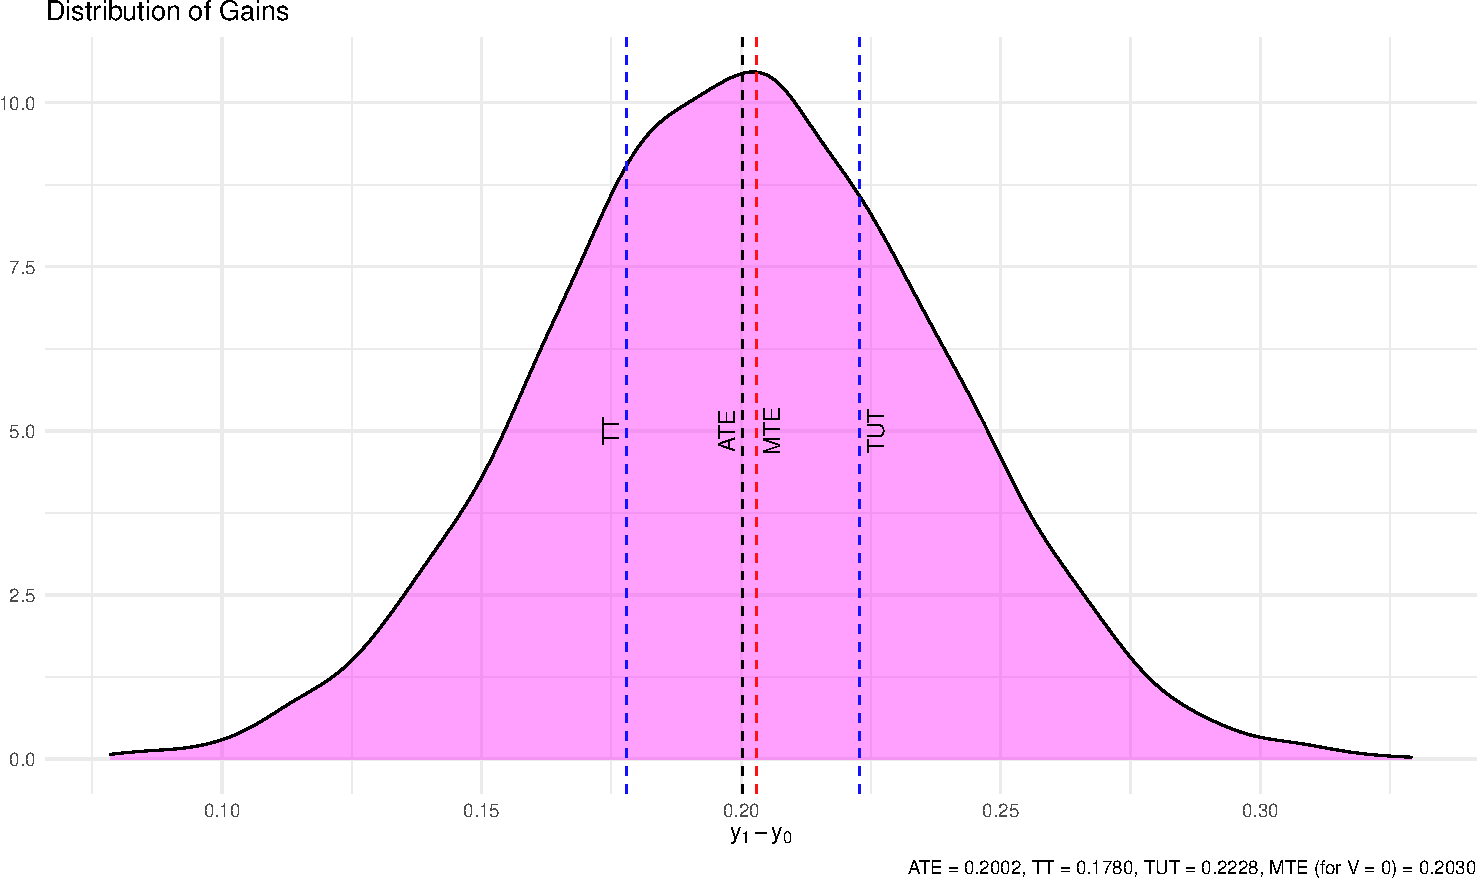
\includegraphics[width=0.85\linewidth,]{hw1_files/figure-latex/unnamed-chunk-2-1} \end{center}

\hypertarget{parametrization-2}{%
\section{Parametrization 2}\label{parametrization-2}}

\begin{Shaded}
\begin{Highlighting}[]
\NormalTok{LATE }\OtherTok{\textless{}{-}} \ControlFlowTok{function}\NormalTok{(param, old, new) \{}
\NormalTok{    Z.old }\OtherTok{\textless{}{-}}\NormalTok{ Z}
\NormalTok{    Z.new }\OtherTok{\textless{}{-}}\NormalTok{ Z}
    
\NormalTok{    Z.old[, param] }\OtherTok{\textless{}{-}}\NormalTok{ old}
\NormalTok{    Z.new[, param] }\OtherTok{\textless{}{-}}\NormalTok{ new}
    
\NormalTok{    I.old }\OtherTok{\textless{}{-}}\NormalTok{ (Z.old }\SpecialCharTok{\%*\%}\NormalTok{ g) }\SpecialCharTok{+}\NormalTok{ V}
\NormalTok{    D.old }\OtherTok{\textless{}{-}} \FunctionTok{ifelse}\NormalTok{(I.old }\SpecialCharTok{\textgreater{}=} \DecValTok{0}\NormalTok{, }\DecValTok{1}\NormalTok{, }\DecValTok{0}\NormalTok{)}
    
\NormalTok{    I.new }\OtherTok{\textless{}{-}}\NormalTok{ (Z.new }\SpecialCharTok{\%*\%}\NormalTok{ g) }\SpecialCharTok{+}\NormalTok{ V}
\NormalTok{    D.new }\OtherTok{\textless{}{-}} \FunctionTok{ifelse}\NormalTok{(I.new }\SpecialCharTok{\textgreater{}=} \DecValTok{0}\NormalTok{, }\DecValTok{1}\NormalTok{, }\DecValTok{0}\NormalTok{)}
    
\NormalTok{    test }\OtherTok{\textless{}{-}} \FunctionTok{ifelse}\NormalTok{((D.old }\SpecialCharTok{==} \DecValTok{0}\NormalTok{) }\SpecialCharTok{\&}\NormalTok{ (D.new }\SpecialCharTok{==} \DecValTok{1}\NormalTok{), }\DecValTok{1}\NormalTok{, }\DecValTok{0}\NormalTok{)}
    
\NormalTok{    temp.df }\OtherTok{\textless{}{-}} \FunctionTok{data.frame}\NormalTok{(}
        \StringTok{\textquotesingle{}beta\textquotesingle{}} \OtherTok{=}\NormalTok{ Y1 }\SpecialCharTok{{-}}\NormalTok{ Y0,}
        \StringTok{\textquotesingle{}test\textquotesingle{}} \OtherTok{=}\NormalTok{ test}
\NormalTok{    )}
    
\NormalTok{    r }\OtherTok{\textless{}{-}}\NormalTok{ temp.df }\SpecialCharTok{\%\textgreater{}\%}
        \FunctionTok{filter}\NormalTok{((test }\SpecialCharTok{==} \DecValTok{1}\NormalTok{)) }\SpecialCharTok{\%\textgreater{}\%}
        \FunctionTok{pull}\NormalTok{(beta) }\SpecialCharTok{\%\textgreater{}\%}
        \FunctionTok{mean}\NormalTok{()}
    
    \FunctionTok{return}\NormalTok{(r)}
\NormalTok{\}}

\NormalTok{regress }\OtherTok{\textless{}{-}} \ControlFlowTok{function}\NormalTok{(beta) \{}
\NormalTok{    intercept }\OtherTok{\textless{}{-}} \FunctionTok{mean}\NormalTok{(Y) }\SpecialCharTok{{-}}\NormalTok{ (beta }\SpecialCharTok{*} \FunctionTok{mean}\NormalTok{(D))}
\NormalTok{    intercept }\SpecialCharTok{+}\NormalTok{ (beta }\SpecialCharTok{*}\NormalTok{ D)}
\NormalTok{\}}
\end{Highlighting}
\end{Shaded}

\hypertarget{latez_1--2-z_1-1}{%
\subsection{\texorpdfstring{\(LATE(z_1 = -2, z'_1 = 1)\)}{LATE(z\_1 = -2, z'\_1 = 1)}}\label{latez_1--2-z_1-1}}

\begin{Shaded}
\begin{Highlighting}[]
\NormalTok{LATE}\FloatTok{.1} \OtherTok{\textless{}{-}} \FunctionTok{LATE}\NormalTok{(}\DecValTok{2}\NormalTok{, }\SpecialCharTok{{-}}\DecValTok{2}\NormalTok{, }\DecValTok{1}\NormalTok{)}
\end{Highlighting}
\end{Shaded}

\(LATE(z_1 = -2, z'_1 = 1) = 0.2051\).

\hypertarget{latez_2-0-z_2-2}{%
\subsection{\texorpdfstring{\(LATE(z_2 = 0, z'_2 = 2)\)}{LATE(z\_2 = 0, z'\_2 = 2)}}\label{latez_2-0-z_2-2}}

\begin{Shaded}
\begin{Highlighting}[]
\NormalTok{LATE}\FloatTok{.2} \OtherTok{\textless{}{-}} \FunctionTok{LATE}\NormalTok{(}\DecValTok{3}\NormalTok{, }\DecValTok{0}\NormalTok{, }\DecValTok{2}\NormalTok{)}
\end{Highlighting}
\end{Shaded}

\(LATE(z_2 = 0, z'_2 = 2) = 0.1982\).

\hypertarget{ivz_1}{%
\subsection{\texorpdfstring{\(IV(Z_1)\)}{IV(Z\_1)}}\label{ivz_1}}

\begin{Shaded}
\begin{Highlighting}[]
\NormalTok{beta.IV.Z1 }\OtherTok{\textless{}{-}}\NormalTok{ (}\FunctionTok{cov}\NormalTok{(Z[, }\DecValTok{2}\NormalTok{], Y) }\SpecialCharTok{/} \FunctionTok{cov}\NormalTok{(Z[, }\DecValTok{2}\NormalTok{], D))[}\DecValTok{1}\NormalTok{, }\DecValTok{1}\NormalTok{]}
\NormalTok{Y.IV.Z1 }\OtherTok{\textless{}{-}} \FunctionTok{regress}\NormalTok{(beta.IV.Z1)}
\end{Highlighting}
\end{Shaded}

\(\hat{\beta}_{\text{IV}} (Z_1) = 0.2045\).

\hypertarget{ivz_2}{%
\subsection{\texorpdfstring{\(IV(Z_2)\)}{IV(Z\_2)}}\label{ivz_2}}

\begin{Shaded}
\begin{Highlighting}[]
\NormalTok{beta.IV.Z2 }\OtherTok{\textless{}{-}}\NormalTok{ (}\FunctionTok{cov}\NormalTok{(Z[, }\DecValTok{3}\NormalTok{], Y) }\SpecialCharTok{/} \FunctionTok{cov}\NormalTok{(Z[, }\DecValTok{3}\NormalTok{], D))[}\DecValTok{1}\NormalTok{, }\DecValTok{1}\NormalTok{]}
\NormalTok{Y.IV.Z2 }\OtherTok{\textless{}{-}} \FunctionTok{regress}\NormalTok{(beta.IV.Z2)}
\end{Highlighting}
\end{Shaded}

\(\hat{\beta}_{\text{IV}} (Z_2) = 0.206\).

\hypertarget{ols}{%
\subsection{\texorpdfstring{\(OLS\)}{OLS}}\label{ols}}

\begin{Shaded}
\begin{Highlighting}[]
\NormalTok{beta.OLS }\OtherTok{\textless{}{-}}\NormalTok{ (}\FunctionTok{cov}\NormalTok{(D, Y) }\SpecialCharTok{/} \FunctionTok{var}\NormalTok{(D))[}\DecValTok{1}\NormalTok{, }\DecValTok{1}\NormalTok{]}
\NormalTok{Y.OLS }\OtherTok{\textless{}{-}} \FunctionTok{regress}\NormalTok{(beta.OLS)}
\end{Highlighting}
\end{Shaded}

\(\hat{\beta}_{\text{OLS}} = 0.237\).

\vspace*{20px}

Given our regression outcomes, the OLS regression shows less variance
than the other estimators, but it is more biased. These results exhibit
the conflict in trying to simultaneously minimize these two sources of
error. Similar estimations, also imply that there is not single best
optimization algorithm as it is stated in the so called \emph{no free
lunch theorem}.

\hypertarget{gmm}{%
\section{GMM}\label{gmm}}

Using \(Z = (Z_1, Z_2)\) as instruments and
\(\displaystyle \hat{V}_0 = \frac{1}{n} \sum_{i = 1}^n z_i' z_i\) as the
weighting matrix, we can estimate our model by the generalized method of
moments.

Hence, we can obtain

\[
\hat{\beta}_{\text{GMM}} = \left( D' Z V_0^{-1} Z' D \right)^{-1} D' Z V_0^{-1} Z' Y.
\]

Note that we can rewrite \(\displaystyle \hat{V}_0 = \frac{1}{n} Z' Z\).

Thus,

\begin{Shaded}
\begin{Highlighting}[]
\NormalTok{subset.Z }\OtherTok{\textless{}{-}}\NormalTok{ Z[, }\SpecialCharTok{{-}}\DecValTok{1}\NormalTok{]}

\NormalTok{V0 }\OtherTok{\textless{}{-}}\NormalTok{ (}\DecValTok{1} \SpecialCharTok{/}\NormalTok{ N) }\SpecialCharTok{*}\NormalTok{ (}\FunctionTok{t}\NormalTok{(subset.Z) }\SpecialCharTok{\%*\%}\NormalTok{ subset.Z)}

\NormalTok{beta.GMM }\OtherTok{\textless{}{-}}
\NormalTok{    (}
        \FunctionTok{solve}\NormalTok{(}\FunctionTok{t}\NormalTok{(D) }\SpecialCharTok{\%*\%}\NormalTok{ subset.Z }\SpecialCharTok{\%*\%} \FunctionTok{solve}\NormalTok{(V0) }\SpecialCharTok{\%*\%} \FunctionTok{t}\NormalTok{(subset.Z) }\SpecialCharTok{\%*\%}\NormalTok{ D) }\SpecialCharTok{\%*\%}
            \FunctionTok{t}\NormalTok{(D) }\SpecialCharTok{\%*\%}\NormalTok{ subset.Z }\SpecialCharTok{\%*\%} \FunctionTok{solve}\NormalTok{(V0) }\SpecialCharTok{\%*\%} \FunctionTok{t}\NormalTok{(subset.Z) }\SpecialCharTok{\%*\%}\NormalTok{ Y}
\NormalTok{    )[}\DecValTok{1}\NormalTok{, }\DecValTok{1}\NormalTok{]}

\NormalTok{Y.GMM }\OtherTok{\textless{}{-}} \FunctionTok{regress}\NormalTok{(beta.GMM)}
\end{Highlighting}
\end{Shaded}

\begin{longtable}[]{@{}lll@{}}
\toprule
Estimator & Estimate & Standard Error \\
\midrule
\endhead
\(\hat{\beta}_{\text{GMM}}\) & 0.2087 & 0.0321 \\
\(\hat{\beta}_{\text{IV}} (Z_1)\) & 0.2045 & 0.0331 \\
\(\hat{\beta}_{\text{IV}} (Z_2)\) & 0.206 & 0.0327 \\
\(\hat{\beta}_{\text{OLS}}\) & 0.237 & 0.0288 \\
\bottomrule
\end{longtable}

\hypertarget{likelihood-function}{%
\section{Likelihood Function}\label{likelihood-function}}

We know that

\begin{align*}
Pr\left(D = 1 \mid Z\right) &= Pr\left(\gamma Z + V \geq 0 \right) \\
&= Pr\left( \frac{-Z\gamma}{\sigma^*_V} \leq \epsilon \right) \\
&= 1 - Pr\left( \epsilon \leq \frac{-Z\gamma}{\sigma^*_V} \right) \\
&= 1 - \Phi \left( \frac{-Z\gamma}{\sigma^*_V} \right),
\end{align*}

and

\begin{align*}
Pr\left(D = 0 \mid Z\right) &= Pr\left(\gamma Z + V < 0 \right) \\
&= Pr\left( \epsilon \leq \frac{-Z\gamma}{\sigma^*_V} \right) \\
&= \Phi \left( \frac{-Z\gamma}{\sigma^*_V} \right).
\end{align*}

Hence,

\begin{align*}
\mathcal{L} &= \prod_{d_i = 0} \left[ \Phi \left( \frac{-Z\gamma}{\sigma^*_v} \right) \right] \prod_{d_i = 1} \left[ 1-  \Phi \left( \frac{-Z\gamma}{\sigma^*_v} \right) \right] \\
&= \prod_{i} \left[ \Phi \left( \frac{-Z\gamma}{\sigma^*_v} \right) \right]^{1 - d_i} \left[ 1-  \Phi \left( \frac{-Z\gamma}{\sigma^*_v} \right) \right]^{d_i},
\end{align*}

and

\begin{align*}
\ell &= \log\mathcal{L} \\
&= \sum_{i} (1 - d_i) \log \left( \Phi \left( \frac{-Z\gamma}{\sigma^*_V} \right) \right) \\
&+ \sum_{i} d_i \log \left( 1 - \Phi \left( \frac{-Z\gamma}{\sigma^*_V} \right) \right) \\
&= \sum_{i} (1 - d_i) \log \left( \Phi \left( \frac{-\gamma_0 - z_1\gamma_1 - z_2\gamma_2}{\sigma^*_V} \right) \right) \\
&+ \sum_{i} d_i \log \left( 1 - \Phi \left( \frac{-\gamma_0 - z_1\gamma_1 - z_2\gamma_2}{\sigma^*_V} \right) \right).
\end{align*}

\hypertarget{discussion}{%
\section{Discussion}\label{discussion}}

The variance on \(V\) (\(\sigma^*_V\)) is not identified and so we
normalize it to 1.

\showmatmethods
\showacknow
\pnasbreak



% Bibliography
% \bibliography{pnas-sample}

\end{document}
